\clearpage
\chapter{}
\section{Genotyping-by-sequencing}
%%%%%%%%%%%%%%%%%%%%%%%%%%%%%%%%%%%%%%%%%%%%%%%%%%%%%%%%%%%%%%%%%%%%%
\addcontentsline{toc}{subsection}{Summary}
\subsection*{SUMMARY}
\hrule
Here is a summary of some results from my GBS analyses.

\begin{table}[ht]
\centering
\caption{Number of variants (SNPs) for the pilot genotyping-by-sequencing run for Lake Tanganyika \textit{Lates} under different alignment and filtering conditions. Individuals were excluded from variant calling if they had fewer than 5,000 reads (5k) or 20,000 reads (20k). Raw SNPs are before filtering for missing data, minor allele frequency, and proximity to other SNPs (90bp threshold); these SNPs have already been filtered using bcftools based on QUAL $>$ 19 and GQ $>$ 9, and only SNPs (not indels or sites with $>$ 2 alleles) have been kept. The labels "with WGS" and "no nilo" refer to datasets containing whole genome re-sequencing data and omitting \textit{Lates niloticus} individuals, respectively.}

\label{table:gbs-stats}
\begin{tabular}{@{}llllll@{}}
\toprule
                 &           &     & \multicolumn{3}{c}{Missing Data Allowed}     \\
Reference Genome & Raw SNPs & MAF & $\leq$ 0.5 & $\leq$ 0.3    & $\leq$ 0.2    \\ \midrule
Lates calcarifer & 4,085,115 & 0.01 & 70,180 & 59,144 & 52,397 \\
                 &           & 0.05 & 33,854 & 28,991 & 25,641 \\ \midrule \midrule
Lates mariae    & 153,175   & 0.01 & 19,025 & 14,542 & 12,091 \\
                 &           & 0.05 & 10,541 & 7,721 & 6,205  \\ \midrule
Lates mariae, no nilo &  139,881  & 0.01 & 17,422 & 13,334 & 10,832 \\
                 &           & 0.05 & 10,527 & 7,845 & 6,318  \\ \midrule
Lates mariae, no nilo, with WGS & 3,076,112 & 0.01 & 22,247 & 14,933 & 12,252 \\
                 &           & 0.05 & 12,438 & 8,388 & 6,770 \\ \midrule
Lates mariae, with WGS (5k) & 3,087,655 & 0.01 & 23,641 & 16,019 & 13,406 \\
                 &           & 0.05 & 12,124 & 8,228 & 6,619 \\ \midrule
Lates mariae, with WGS (20k) & 3,086,364 & 0.01 & 24,907 & 17,275 & 14,619 \\
                 &           & 0.05 & 13,002 & 8,898 & 7,398 \\
\bottomrule
\end{tabular}
\end{table}

%%%%%%%%%%%%%%%%%%%%%%%%%%%%%%%%%%%%%%%%%%%%%%%%%%%%%%%%%%%%%%%%%%%%%
\subsection*{NEXT TO-DO}
\hrule

\begin{enumerate}
\item Item 1
\end{enumerate}
%%%%%%%%%%%%%%%%%%%%%%%%%%%%%%%%%%%%%%%%%%%%%%%%%%%%%%%%%%%%%%%%%%%%%
\addcontentsline{toc}{subsection}{Log}
\subsection*{LOG}
\hrule

%%%%%%%%%%%%%%%%%%
\hrulefill
\begin{large}\textbf{24 Feb 2018}\end{large} \\
%%%%%%%%%%%%%%%%%%
An entry from Feb 24th, with a figure (Fig. \ref{fig:cutsite-locations}).

%% FIGURE %%
\begin{figure}[ht]
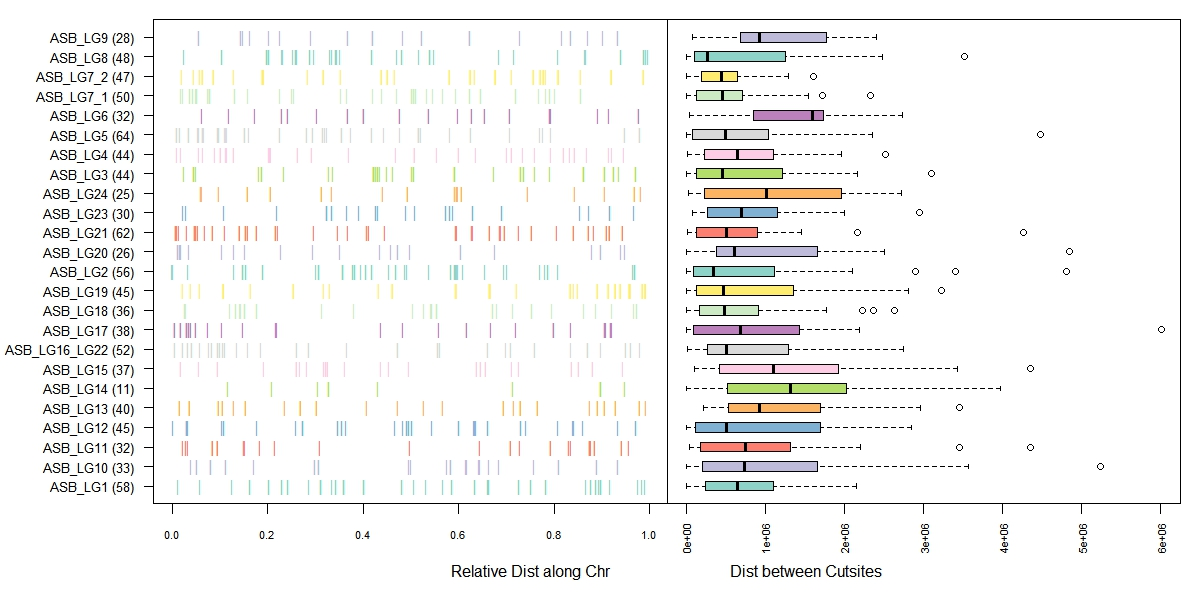
\includegraphics[width=0.9\textwidth]
{figures/insilico_cutsite_locations.jpeg}\caption{\label{fig:cutsite-locations} Plot of the location of cutsites shared by the GBS and RAD methods (where cutsites for SbfI occur within 150bp of a location where EcoRI and MseI cutsites fall within our size selection criteria of 200-350bp). Left-hand panel shows the spacing of potential shared SNPs along the chromosomes. Right-hand panel shows boxplots of the distances between these potential SNP locations, to give an idea of how useful these potential shared SNPs may be.}
\end{figure}
%%%%

%%%%%%%%%%%%%%%%%%%%%%%%%%%%%%%%%%%%%%%%%%%%%%%%%%%%%%%%%%%%%%%%%%%%%
\addcontentsline{toc}{subsection}{Third subsection}
\subsection*{ANOTHER SUBSECTION}
\hrule
Here are some details in another subsection of information.
%%%%%%%%%%%%%%%%%%%%%%%%%%%%%%%%%%%%%%%%%%%%%%%%%%%%%%%%%%%%%%%%%%%%%
\bibliographystyle{agsm}
\bibliography{Mendeley_022218}

